\section{Applications of TeraHeap}

In this section, we describe how we integrate \teraheapName{} with two widely-used
frameworks, Spark~\cite{zaharia:spark} and Giraph~\cite{giraph}, which differ
significantly in their use of off-heap memory. Spark operates with immutable
objects, which presents a simpler scenario for \teraheapName{}, as immutability avoids
the complexities of managing object mutations. In contrast, Giraph involves more
complex mutation processes, requiring expensive read-modify-write operations to
the storage device when moving updated objects off-heap. In the context of
\teraheapName{}, these updates increase backward references from H2 to H1. This increase
in cross-heap references stresses the \teraheapGC{} process, as the \teraheapGC{} must track and
manage these references. Additionally, we explore the application of \teraheapName{} in
Neo4j's-GDS library~\cite{gds}, which cannot move objects in off-heap memory.
Our approach enables GDS to handle problem sizes that exceed the limitations of
DRAM.

\subsection{Analytics Frameworks with Off-heap Support}

Spark uses off-heap memory to cache intermediate results, avoiding
expensive recomputation. Cached objects are immutable at allocation
time. Unlike Spark, Giraph offloads mutable objects, i.e., vertices,
edges, and messages, to off-heap memory to ensure adequate DRAM is
available for each superstep. Giraph updates vertex values throughout
the computation, whereas edges and messages become immutable after
graph loading (edges) or at the end of a superstep (messages).

Spark users explicitly annotate objects that need to be moved off-heap
with the \texttt{persist()} call. Giraph transparently selects and
moves objects to the storage device without application interaction.
It maintains an \emph{out-of-core} scheduler that monitors memory
pressure in the managed heap and decides which vertices, edges, and
messages to move off-heap. The out-of-core scheduler selects based on
a least recently used policy which objects to move off-heap.

Spark maintains deserialized objects in memory. This incurs
significant \teraheapSD overhead during the off-heap movement. Giraph tries
to reduce memory consumption on the managed heap and serializes
vertices, edges, and messages into byte arrays, at allocation time.
Therefore, Giraph does not require \teraheapSD when moving these byte arrays
off-heap on the storage device.
%
Next, we discuss how we extend Spark and Giraph to use \teraheapName{}.

\begin{figure}[t]
	\centering
  \subfloat[]{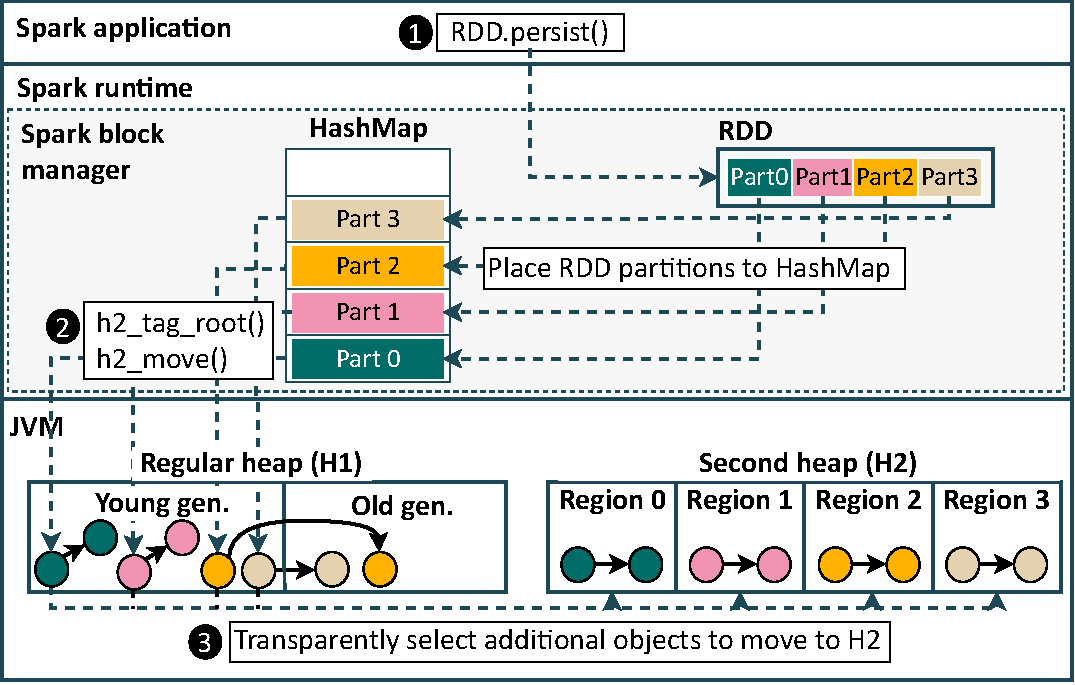
\includegraphics[width=0.49\linewidth]{teraheap/fig/teracache_diag-crop.pdf}}
  \hspace{5pt}
  \subfloat[]{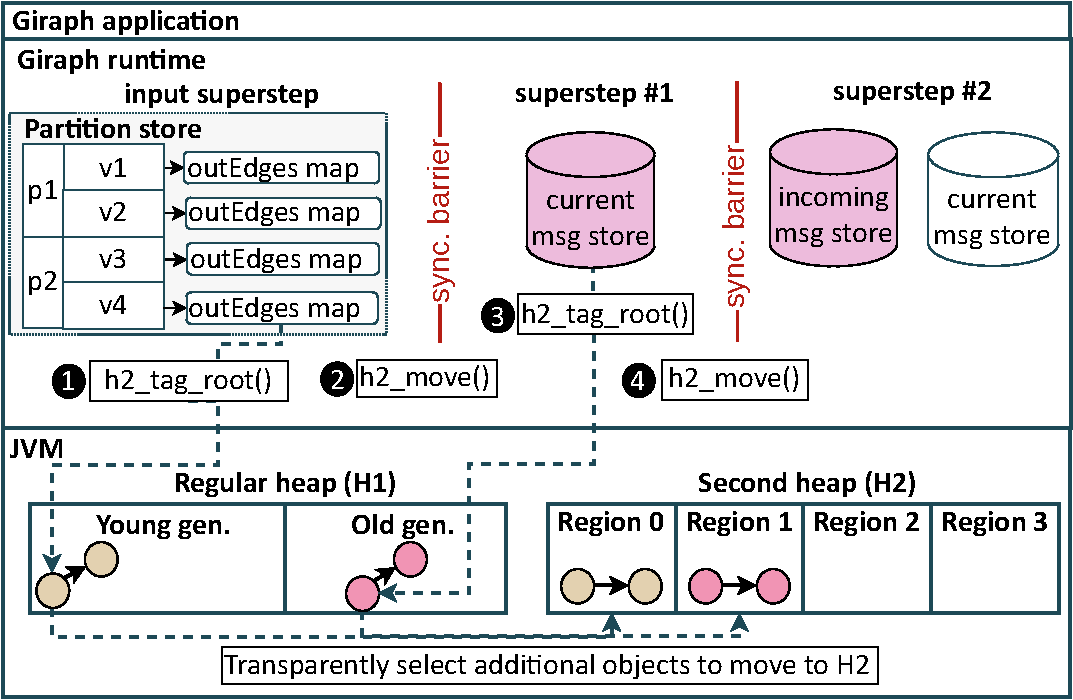
\includegraphics[width=0.48\linewidth]{teraheap/fig/giraph-crop.pdf}}
  \caption{Use of TeraHeap in (a) Spark and (b) Giraph.}
	\label{fig:spark_diag}
\end{figure}

\paragraph{\textbf{Spark}}

We examine the use of \teraheapName{} as an on-heap compute cache in Spark.
Spark requires only slight modifications to use \teraheapName{}. We note that
Spark abstracts intermediate results as immutable collections using
three sets of APIs~\cite{spark:apis}: resilient distributed datasets
(RDDs)~\cite{rdd}, DataFrames, and Datasets. To avoid
time-consuming~\cite{Xu:Neutrino} recomputation of commonly used
intermediate results across different jobs, Spark offers the
flexibility of caching RDDs, Dataframes, or Datasets via its
\emph{persist()} API~\cite{rdd}. Users can persist RDDs,
Dataframes, or Datasets in different storage levels: memory (on-heap),
disk (off-heap), or both.
%
When an RDD, Dataframe, or Dataset partition does not fit in storage
memory, Spark serializes (e.g., using Kryo~\cite{kryo}) and moves
another partition to a storage device, using a Least Recently Used
(LRU) policy. To use \teraheapName{}, we simply mark all cached partitions
of RDDs, DataFrames, or Datasets, as root objects for moving to H2.

Figure~\ref{fig:spark_diag}(a) shows the flow of Spark
caching operations using \teraheapName{}:
%
\teraheapCircled{1} The application code invokes \texttt{persist()} without any
modifications.
%
\teraheapCircled{2} The Spark block manager places the selected data in the
compute cache, a hashmap that contains all cached partitions. The
block manager caches each partition independently, maintaining
per-partition entries in the hashmap. When the block manager stores a
new partition in the hashmap, we mark the partition descriptor as a
root key-object with the \texttt{h2\_tag\_root()}, providing as label
the RDD, dataset, or dataframe id. At the same time, we advise JVM to
move marked partitions to H2, using \texttt{h2\_move()}.
\teraheapName{} allows Spark to cache all RDDs on-heap without
replacing the Spark block manager.
%
\teraheapCircled{3} \teraheapName{} transparently marks additional objects and moves
them to H2 during the major \teraheapGC.

\paragraph{\textbf{Giraph}}
Giraph computes in supersteps, with a synchronization barrier between
supersteps. It loads and partitions the graph during the input
superstep.  A graph partition organizes its vertices in a hashmap,
with each vertex belonging to a single partition. Each vertex
maintains a map containing its outgoing edges. In each superstep, each
vertex consumes all of its incoming messages from the previous
superstep and updates its value.  Then, it sends its updated value to
its outgoing edges in a new message (per vertex). Messages produced in
the current superstep are only consumed in the next superstep.
Messages become immutable at the end of each superstep after the
coordination phase guarantees they have been received and saved
completely.  In each superstep, Giraph has two message stores: the
\emph{incoming message store} with messages from the previous
superstep (immutable) and the \emph{current message store} with
messages of the current superstep (mutable).

To use \teraheapName, Giraph requires small modifications, as well. We extend
Giraph by marking edges and incoming messages as root objects. We do
not mark vertices because they have frequent updates, and they will
increase device (write) traffic. Note that edges and messages
constitute a large portion of the heap~\cite{giraph}.
Figure~\ref{fig:spark_diag}(b) shows the  flow of Giraph execution using
\teraheapName{}:
%
\teraheapCircled{1} When Giraph loads a new vertex at the input superstep, it
marks the vertex's map that contains the outgoing edges with
\texttt{h2\_tag\_root()}, providing the superstep id as label.
%
\teraheapCircled{2} At the end of the input superstep, Giraph advises \teraheapName{}
to move marked edges to H2, using \texttt{h2\_move()} in the next major
\teraheapGC.
%
\teraheapCircled{3} In each superstep, Giraph marks the generated messages of
the  current message store with \texttt{h2\_tag\_root()}, providing as
label the superstep id.
%
\teraheapCircled{4} At the beginning of each (next) superstep, Giraph advises
\teraheapName{} to move to H2 all marked messages from the previous superstep
in the next major \teraheapGC, using \texttt{h2\_move()}.

\subsection{Analytics Frameworks without Off-Heap Support}
We aim to demonstrate the effectiveness of \teraheapName{} in analytics frameworks that
lack support for offloading objects off-heap. GDS is a library for the Neo4j
graph database, which provides many graph algorithms that can be used to analyze
and extract insights from the graph stored in the database. GDS loads the graph
data into memory by representing the graph as a compressed sparse row (CSR)
format to reduce its size. Although this technique can reduce memory demands, it
becomes less space efficient as the graph size increases~\cite{neo4j:ssd}.

\begin{figure}[t]
	\centering
	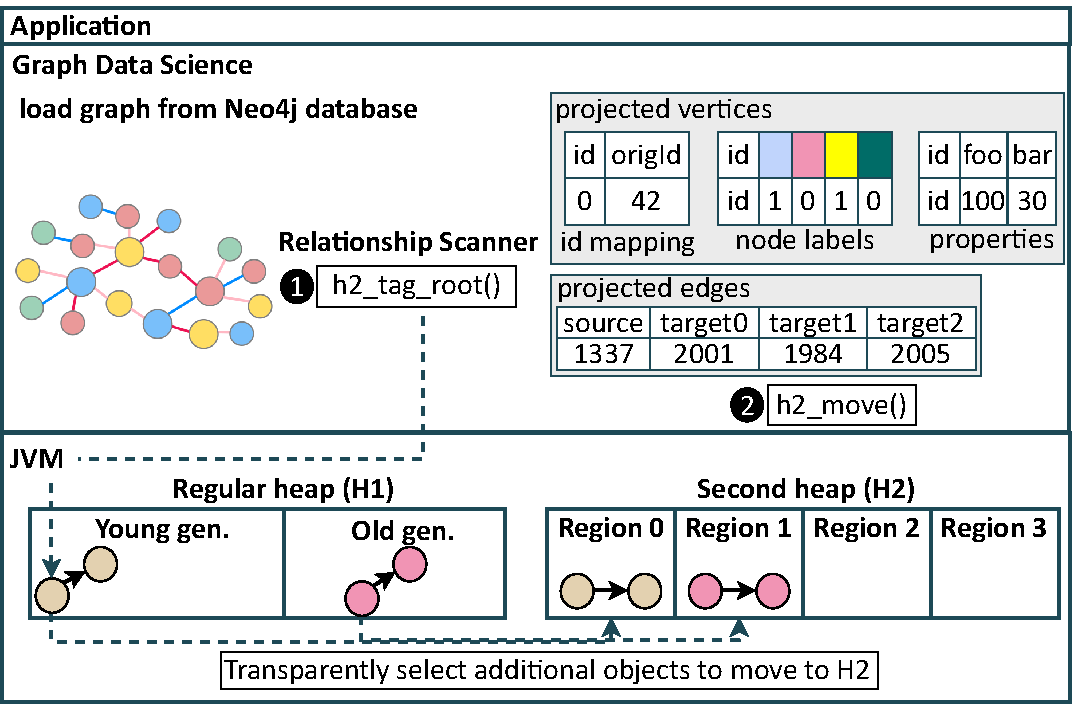
\includegraphics[width=0.6\linewidth]{teraheap/fig/gds.pdf}
  \caption{Use of TeraHeap in Graph Data Science of Neo4j.}
	\label{fig:gds}
\end{figure}

Enabling the GDS to use \teraheapName{} requires inserting the hints in the GDS source
code, which involves modification to two lines of code. \teraheapName{} does not change
the CSR format of the graph in memory and allows GDS to operate in the usual
manner. Importantly, it imposes no limitations on the operations that GDS
perform over the graph. Figure~\ref{fig:gds} shows the flow of GDS using
\teraheapName{}.
%
\teraheapCircled{1} Using a cypher query, GDS loads the graph from the Neo4j
database. GDS uses \texttt{h2\_tag\_root()} to mark vertices and edges
by providing as a label the thread ID.
%
\teraheapCircled{2} After creating the projected graph representation
in memory, GDS uses \texttt{h2\_move()} to advise \teraheapName{} to move all
vertices and edges to the H2. After that, it continues the normal execution
path.

\subsection{Applicability to Other Frameworks}

Given that \teraheapName{} is a JVM-level solution, higher layers can use \teraheapName{}
transparently by only providing simple hints. The API of \teraheapName{} can be adopted
by any big data framework that creates objects that span multiple computation
steps and require a large amount of memory. Such frameworks include
Hadoop~\cite{hadoop}, Flink~\cite{flink}, search engines like
Lucene~\cite{lucene}, or database systems such as Cassandra~\cite{teraheap:cassandra}.
For example, Lucene~\cite{lucene} allocates its query cache on the heap, where
frequently executed queries are stored to avoid recomputation. However,
managing the query cache size can significantly impact \teraheapGC{}. To mitigate this
issue, Lucene can utilize the hint-based interface of \teraheapName{}, enabling the
allocation of its query cache to H2, thus optimizing performance. Similarly,
Cassandra~\cite{teraheap:cassandra}, which traditionally stores cached rows off-heap,
could further enhance its efficiency by leveraging \teraheapName{} to transfer cached
rows to H2, incorporating specific API calls directly into its codebase for
seamless integration.
